\chapter{fMRI model estimation \label{Chap:fmri_est}}

Model parameters can be estimated using classical (ReML - Restricted Maximum Likelihood) or Bayesian algorithms. After parameter estimation, the RESULTS button can be used to specify contrasts that will produce Statistical Parametric Maps (SPMs), Effect Size Maps (ESMs) or Posterior Probability Maps (PPMs) and tables of statistics. 

\section{Select SPM.mat}

Select the \texttt{SPM.mat} file that contains the design specification. SPM will output the results of its analysis into this directory. This includes overwriting the \texttt{SPM.mat} file. When the estimation job is run, no warning will be given that the SPM.mat file will be overwritten. A warning is given at the specification stage. When it comes to estimation, SPM assumes that you've now sorted out your directory structures.

\begin{figure}
\begin{center}
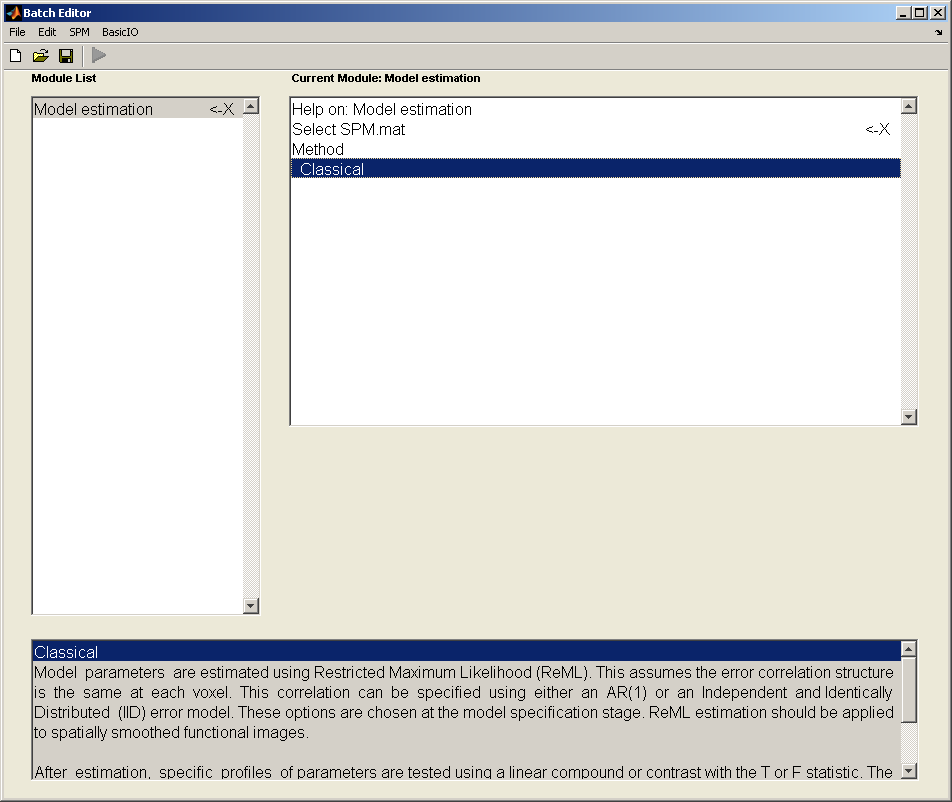
\includegraphics[width=100mm]{fmri_est/est_method}
\end{center}
\caption{\em After starting SPM in fMRI mode and pressing the ``Estimate'' button, the SPM batch editor window should appear as above. The options for ``fMRI model estimation'' can be examined by clicking on them. A single click will bring up some help text in the lower subwindow (not shown in the above graphic). Options highlighted with a `$<$-X' are mandatory and must be filled in by the user. Each of the options shown above is described in this chapter. \label{est}}
\end{figure}

\section{Method}

There are three possible estimation procedures for fMRI models (1) classical (ReML) estimation of first or second level models, (2) Bayesian estimation of first level models and (3) Bayesian estimation of second level models. Option (2) uses a Variational Bayes (VB) algorithm introduced in SPM5. Option (3) uses the Empirical Bayes algorithm with global shrinkage priors that was also in SPM2.

To use option (3) you must have already estimated the model using option (1). That is, for second-level models you must run a ReML estimation before running a Bayesian estimation. This is not necessary for option (2). Bayesian estimation of 1st-level models using VB does not require a prior ReML estimation.

\subsection{Classical}

Model parameters are estimated using Restricted Maximum Likelihood (ReML). This assumes the error correlation structure is the same at each voxel. This correlation can be specified using either an AR(1) or an Independent and Identically Distributed (IID) error model. These options are chosen at the model specification stage. ReML estimation should be applied to spatially smoothed functional images. See \cite{peb1,peb2} for further details of the ReML estimation scheme. After estimation, specific profiles of parameters are tested using a linear compound or contrast with the T or F statistic. The resulting statistical map constitutes an SPM. The SPM{T}/{F} is then characterised in terms of focal or regional differences by assuming that (under the null hypothesis) the components of the SPM (ie. residual fields) behave as smooth stationary Gaussian fields.

The rest of this chapter describes the Bayesian estimation options. So, please skip to the next chapter if you are interested only in classical estimation and inference. 

\subsection{Bayesian 1st-level}

Model parameters are estimated using Variational Bayes (VB). This allows you to specify spatial priors for regression coefficients and regularised voxel-wise AR(P) models for fMRI noise processes. The algorithm does not require functional images to be spatially smoothed. Estimation will take about 5 times longer than with the classical approach. This is why VB is not the default estimation option. The VB approach has been described in a number of papers \cite{vb_fmri_ar,vb2,vb3,will_bayes_srglm}.

After estimation, contrasts are used to find regions with effects larger than a user-specified size eg. 1 per cent of the global mean signal. These effects are assessed statistically using a Posterior Probability Map (PPM) \cite{karl_posterior}.

\begin{figure}
\begin{center}
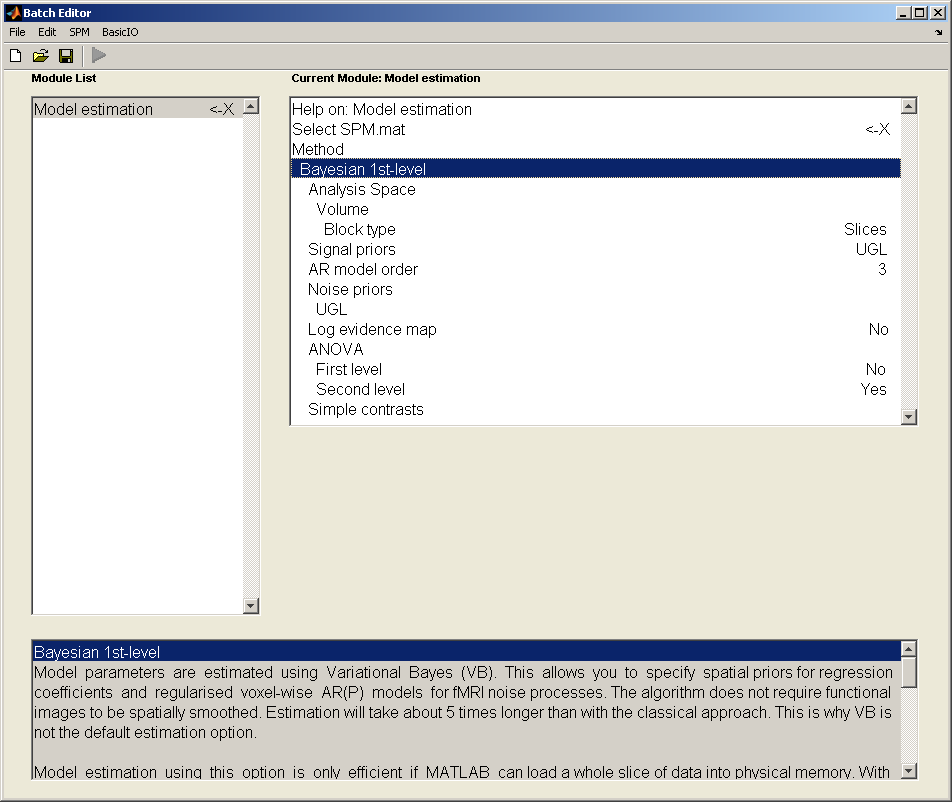
\includegraphics[width=100mm]{fmri_est/bayes_options}
\end{center}
\caption{\em After choosing ``Bayesian 1st-level'' under ``Method'', the SPM batch editor window should appear as above. Each of the options shown above is described in this chapter. \label{bayes_options}}
\end{figure}

\subsubsection{Analysis Space}

Because estimation can be time consuming options are provided to analyse selected slices or clusters rather than the whole volume.

\paragraph{Volume}

A volume of data is analysed in ``blocks'', which can be a slice or 3D subvolume, where the extent of each subvolume is determined using a graph partitioning algorithm. Enter the block type, i.e. ``Slices'' or ``Subvolumes''.

\subparagraph{Block type}

Enter the block type, i.e. ``Slices'' or ``Subvolumes''.

\paragraph{Slices}

Enter Slice Numbers. This can be a single slice or multiple slices. If you select a single slice or only a few slices you must be aware of the interpolation options when, after estimation, displaying the estimated images eg. images of contrasts or AR maps. The default interpolation option may need to be changed to nearest neighbour (NN) (see bottom right hand of graphics window) for you slice maps to be visible.

\subparagraph{Slice numbers}

Enter Slice Numbers.

\subparagraph{Block type}

Enter the block type, i.e. ``Slices'' or ``Subvolume''.

\paragraph{Clusters}

Because estimation can be time consuming an option is provided to analyse selected clusters rather than the whole volume.

\subparagraph{Cluster mask}

Select cluster image.

\subparagraph{Block type}

Enter the block type, i.e. ``Slices'' or ``Subvolumes''.

\subsubsection{Signal priors}
\begin{itemize}
\item \textbf{[UGL] Unweighted Graph Laplacian.} This spatial prior is the recommended option. Regression coefficients at a given voxel are (softly) constrained to be similar to those at nearby voxels. The strength of this constraint is determined by a spatial precision parameter that is estimated from the data. Different regression coefficients have different spatial precisions allowing each putative experimental effect to have its own spatial regularity. 

\item \textbf{[GMRF] Gaussian Markov Random Field.} This is equivalent to a normalized UGL.

\item \textbf{[LORETA] Low resolution Tomography Prior.} This is equivalent to UGL squared. It is a standatd choice for EEG source localisation algorithms.

\item \textbf{[WGL] Weighted Graph Laplacian.} This is a generalization of the UGL, where weights can be used to preserve ``edges'' of functional responses.

\item \textbf{[Global] Global Shrinkage prior.} This is not a spatial prior in the sense that regression coefficients are constrained to be similar to neighboring voxels. Instead, the average effect over all voxels (global effect) is assumed to be zero and all regression coefficients are shrunk towards this value in proporation to the prior precision. This is the same prior that is used for Bayesian estimation at the second level models, except that here the prior precision is estimated separaetly for each slice.

\item \textbf{[Uninformative] A flat prior.} Essentially, no prior information is used. If you select this option then VB reduces to Maximum Likelihood (ML)estimation. This option is useful if, for example, you do not wish to use a spatial prior but wish to take advantage of the voxel-wise AR(P) modelling of noise processes. In this case, you would apply the algorithm to images that have been spatially smoothed. For P=0, ML estimation in turn reduces to Ordinary Least Squares (OLS) estimates, and for P$>$0 ML estimation is equivalent to a weighted least squares (WLS) but where the weights are different at each voxel (reflecting the different noise correlation at each voxel).
\end{itemize}

\subsubsection{AR model order}

An AR model order of 3 is the default. Cardiac and respiratory artifacts are periodic in nature and therefore require an AR order of at least 2. In previous work, voxel-wise selection of the optimal model order showed that a value of 3 was the highest order required. 

Higher model orders have little effect on the estimation time. If you select a model order of zero this corresponds to the assumption that the errors are IID. This AR specification overrides any choices that were made in the model specification stage.

Voxel-wise AR models are fitted separately for each session of data. For each session this therefore produces maps of AR(1), AR(2) etc coefficients in the output directory.

\subsubsection{Noise priors}

There are five noise prior options here (1) UGL, (2) GMRF, (3) LORETA, (4) Tissue-type and (5) Robust.

\paragraph{UGL}

[UGL] Unweighted graph-Laplacian. This is the default option. This spatial prior is the same as that used for the regression coefficients. Spatial precisions are estimated separately for each AR coefficient eg. the AR(1) coefficient over space, AR(2) over space etc. 

\paragraph{GMRF}

[GMRF] Gaussian Markov Random Field. See comments on GMRF priors for regresion coefficients.

\paragraph{LORETA}

[LORETA] Low resolution Tomography Prior. See comments on LORETA priors for regresion coefficients.

\paragraph{Tissue-type}

[Tissue-type] AR estimates at each voxel are biased towards typical values for that tissue type (eg. gray, white, CSF). If you select this option you will need to then select files that contain tissue type maps (see below). These are typically chosen to be Grey Matter, White Matter and CSF images derived from segmentation of registered structural scans.

Previous work has shown that there is significant variation in AR values with tissue type. However, GMRF priors have previously been favoured by Bayesian model comparison.

\paragraph{Robust}

Robust GLM. Uses Mixture of Gaussians noise model.

\subsubsection{Log evidence map}

Computes the log evidence for each voxel

\subsubsection{ANOVA}

Perform 1st or 2nd level Analysis of Variance.

\paragraph{First level}

This is implemented using Bayesian model comparison. For example, to test for the main effect of a factor two models are compared, one where the levels are represented using different regressors and one using the same regressor. This therefore requires explicit fitting of several models at each voxel and is computationally demanding (requiring several hours of computation). The recommended option is therefore NO.

To use this option you must have already specified your factorial design during the model specification stage.

\paragraph{Second level}

This option tells SPM to automatically generate the simple contrasts that are necessary to produce the contrast images for a second-level (between-subject) ANOVA. Naturally, these contrasts can also be used to characterise simple effects for each subject.

With the Bayesian estimation option it is recommended that contrasts are computed during the parameter estimation stage (see 'simple contrasts' below). The recommended option here is therefore YES.

To use this option you must have already specified your factorial design during the model specification stage. 

If you wish to use these contrast images for a second-level analysis then you will need to spatially smooth them to take into account between-subject differences in functional anatomy ie. the fact that one persons V5 may be in a different position than anothers.

\subsubsection{Simple contrasts}

``Simple'' contrasts refers to a contrast that spans one-dimension ie. to assess an effect that is increasing or decreasing.

If you have a factoral design then the contrasts needed to generate the contrast images for a 2nd-level ANOVA (or to assess these simple effects within-subject) can be specified automatically using the ANOVA-$>$Second level option.

When using the Bayesian estimation option it is computationally more efficient to compute the contrasts when the parameters are estimated. This is because estimated parameter vectors have potentially different posterior covariance matrices at different voxels and these matrices are not stored. If you compute contrasts post-hoc these matrices must be recomputed (an approximate reconstruction based on a Taylor series expansion is used). It is therefore recommended to specify as many contrasts as possible prior to parameter estimation.

If you wish to use these contrast images for a second-level analysis then you will need to spatially smooth them to take into account between-subject differences in functional anatomy ie. the fact that one persons V5 may be in a different position than anothers. 

\paragraph{Simple contrast}

\subparagraph{Name}
Name of contrast eg. ``Positive Effect''.

\subparagraph{Contrast vector}
These contrasts are used to generate PPMs which characterise effect sizes at each voxel. This is in contrast to SPMs in which eg. maps of t-statistics show the ratio of the effect size to effect variability (standard deviation). SPMs are therefore a-dimensional. This is not the case for PPMs as the size of the effect is of primary interest. Some care is therefore needed about the scaling of contrast vectors. For example, if you are interested in the differential effect size averaged over conditions then the contrast 0.5 0.5 -0.5 -0.5 would be more suitable than the 1 1 -1 -1 contrast which looks at the differential effect size summed over conditions.

\subsection{Bayesian 2nd-level}

Bayesian estimation of 2nd level models. This option uses the Empirical Bayes algorithm with global shrinkage priors that was previously implemented in SPM2. Use of the global shrinkage prior embodies a prior belief that, on average over all voxels, there is no net experimental effect. Some voxels will respond negatively and some positively with a variability determined by the prior precision. This prior precision can be estimated from the data using Empirical Bayes.

\section{Output files}

After estimation a number of files are written to the output directory. These are

\begin{itemize}
\item{An \verb!SPM.mat! file containing specification of the design and estimated model parameters}
\end{itemize}

\subsection{Classical 1st-level}

For classical 1st-level models the following files are also produced

\begin{itemize}

\item{Images of estimated regression coefficients  \verb!beta_000k.img! where $k$ indexes the $k$th regression coefficient.}

\item{An image of the variance of the error \verb!ResMS.img!.}

\item{An image \verb!mask.img! indicating which voxels were included in the analysis.}

\item{The image \verb!RPV.img!, the estimated resels per voxel.}

\item{If contrasts have been specified SPM also writes \verb!con_000i.img!  if the $i$th contrast is a t-contrast and the extra sum of squares image \verb!ess_000i.img! if it is an F-contrast.} 

\end{itemize}

Type \verb!help spm_spm! at the matlab command prompt for further information.

\subsection{Bayesian 1st-level}

For Bayesian 1st-level models the following files are also produced

\begin{itemize}

\item{Images of estimated regression coefficients  \verb!Cbeta_000k.img! where $k$ indexes the $k$th regression coefficient. These filenames are prefixed with a ``C'' indicating that these are the mean values of the `Conditional' or `Posterior' density.}

\item{Images of error bars/standard deviations on the regression coefficients \verb!SDbeta_000k.img!.}

\item{An image of the standard deviation of the error \verb!Sess1_SDerror.img!.}

\item{An image \verb!mask.img! indicating which voxels were included in the analysis.}

\item{If a non-zero AR model order is specified then SPM also writes images \verb!Sess1_AR_000p.img! where $p$ indexes the $p$th AR coefficient.}

\item{If contrasts have been specified SPM also writes \verb!con_000i.img! and \verb!con_sd_000i.img! which are the mean and standard deviation of the $i$th pre-defined contrast.}

\end{itemize}

Each of these images can be inspected using the ``Display'' button. Type \verb!help spm_spm_vb! at the \matlab\ command prompt for further information.

\section{Model comparison}

Once you have estimated a model you can use SPM's results button to look at the results. You can also extract fMRI data from regions of interest using the ROI button. You can then compare GLMs based on different hemodynamic basis sets using the Bayesian model evidence.

This is described in \cite{will_bayes_srglm} and implemented using the command line option \texttt{spm\_vb\_roi\_basis}. This requires a VOI filename (created using the ROI button) and an SPM data structure. Type \texttt{help spm\_vb\_roi\_basis} at the \matlab\ command prompt for further information. Figure~\ref{basis} shows an example output from the function indicating that, for the data in this brain region, an informed basis set has the highest model evidence.

\begin{figure}
\begin{center}
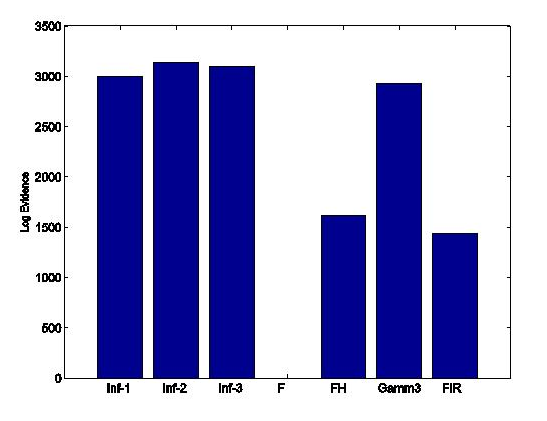
\includegraphics[width=150mm]{fmri_est/basis}
\end{center}
\caption{\em This plot shows the model evidence for a number of different hemodynamic basis sets: Inf1 - Canonical HRF, Inf2 - Canonical plus temporal derivative, Inf3 - Canonical plus temporal and dispersion derivatives, F - Fourier, FH - Fourier with a Hanning Window, Gamm3 - 3 Gamma basis functions and FIR - a Finite Impulse Response function. An informed basis set provides the best model of the data for the selected region.  \label{basis}}
\end{figure}
